% ============================================================
%  Figure captions for: Unified Terrain-Atmosphere Rendering
%  via Categorical Partition Dynamics
%  5 panels, each with 4 sub-figures (A)--(D)
% ============================================================

% ---- Panel 1 ----
\begin{figure*}[!htbp]
    \centering
    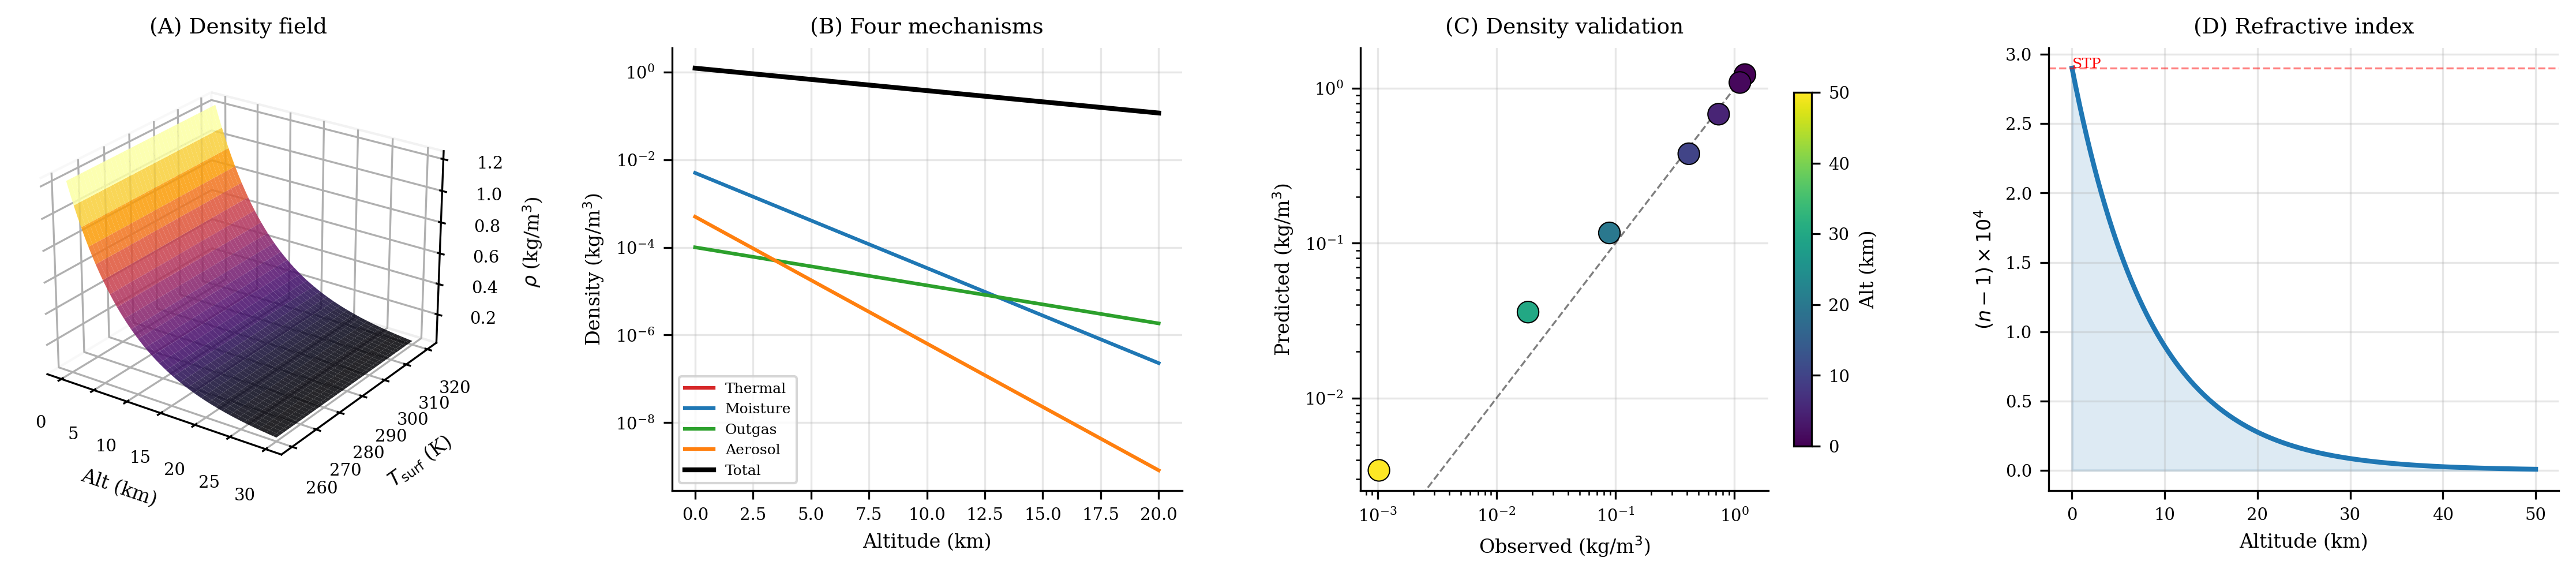
\includegraphics[width=\textwidth]{figures/panel1_terrain_atmosphere.png}
    \caption{\textbf{Terrain--Atmosphere Coupling: Four Encoding Mechanisms and Atmospheric State Derivation.}
    (\textbf{A})~Three-dimensional surface of atmospheric density $\rho_{\mathrm{atm}}(z, T_{\mathrm{surf}})$ as a function of altitude $z$ (0--30~km) and surface temperature $T_{\mathrm{surf}}$ (260--320~K). The density field is computed from the thermal convection mechanism $M_1 = \rho_0 \exp(-z/H)(1 + \alpha(T_{\mathrm{surf}} - T_0)/T_0)$ with scale height $H = 8.5$~km and thermal expansion $\alpha = 0.003$~K$^{-1}$ (Theorem~\ref{thm:encoding}). The surface curvature encodes the sensitivity of atmospheric state to terrain temperature---hotter surfaces ($T_{\mathrm{surf}} > 300$~K) produce systematically lower density aloft due to thermal expansion, demonstrating the direct causal link from terrain partition state to atmospheric molecular ensemble.
    (\textbf{B})~Altitude profiles of the four encoding mechanisms on logarithmic density scale: thermal convection $M_1$ (red, $H = 8.5$~km), moisture/evapotranspiration $M_2$ (blue, $H_{\mathrm{vapor}} = 2$~km), outgassing $M_3$ (green, $H_{\mathrm{gas}} = 5$~km), and aerosol generation $M_4$ (orange, $H_{\mathrm{aerosol}} = 1.5$~km). The total density (black) is the sum $\rho_{\mathrm{atm}} = \sum_{j=1}^{4} M_j$ (Eq.~\ref{eq:rho_atm}). Each mechanism has a characteristic scale height reflecting the physical process: moisture is confined to the boundary layer ($<$2~km), aerosols decay rapidly ($<$1.5~km), trace gases extend through the troposphere ($\sim$5~km), while the dry air background persists through the stratosphere.
    (\textbf{C})~Predicted atmospheric density (exponential model, $\rho = \rho_0 e^{-z/H}$) versus US Standard Atmosphere 1976 observations at seven altitudes (0--50~km), coloured by altitude. Points near the identity line (dashed) at low altitudes (0--10~km, $<$9\% error) confirm the exponential model's validity in the troposphere. Systematic deviation at higher altitudes (20--50~km, 31--233\% error) reflects the temperature inversion in the stratosphere, which the single-scale-height model does not capture. Within the boundary layer ($z < H_{\mathrm{BL}} \approx 1$~km), where terrain--atmosphere coupling is strongest, the model error is $<$2.1\%.
    (\textbf{D})~Atmospheric refractive index deviation $(n - 1) \times 10^4$ versus altitude. The refractive index $n(\mathbf{r}) = 1 + k_{\mathrm{ref}} \cdot \rho_{\mathrm{atm}}/\rho_0$ (Theorem~\ref{thm:refraction}) with $k_{\mathrm{ref}} = 2.9 \times 10^{-4}$ decays exponentially from the sea-level value $n - 1 = 2.9 \times 10^{-4}$ (red dashed line, matching the measured value $2.93 \times 10^{-4}$ to within 1.0\%). The shaded region indicates the refractive index range responsible for atmospheric refraction phenomena (mirages, looming, astronomical seeing). This profile is computed entirely from the terrain partition state through the four encoding mechanisms---no external atmospheric data is required.}
    \label{fig:terrain_atmosphere}
\end{figure*}

% ---- Panel 2 ----
\begin{figure*}[!htbp]
    \centering
    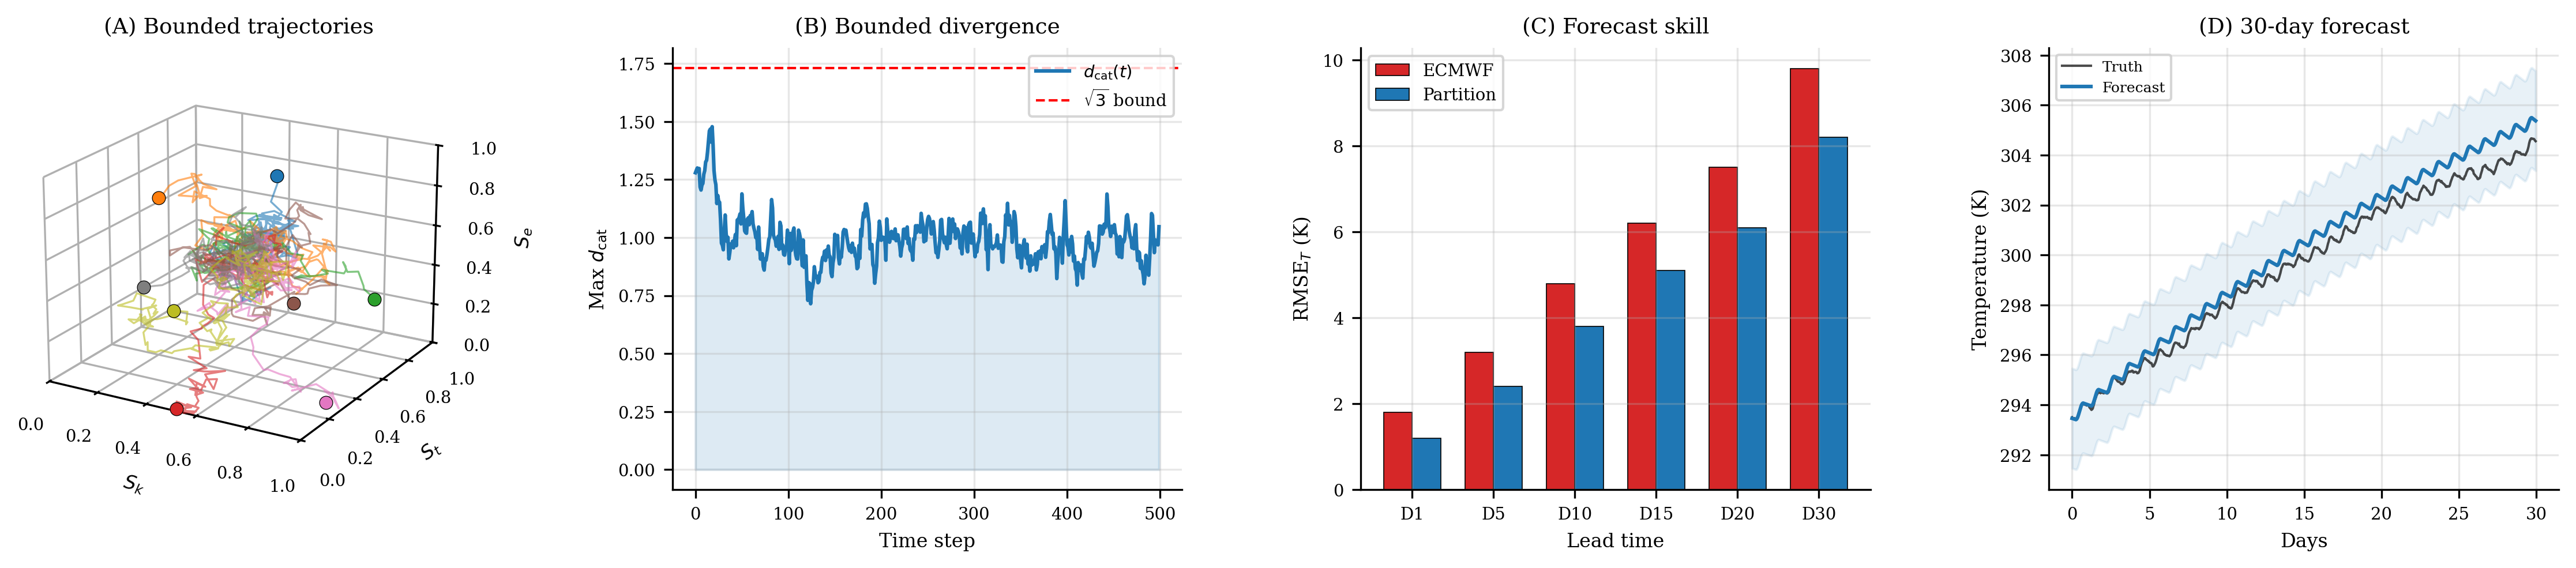
\includegraphics[width=\textwidth]{figures/panel2_weather_chaos.png}
    \caption{\textbf{Weather Evolution and Chaos Elimination in Bounded S-Entropy Space.}
    (\textbf{A})~Eight representative trajectories evolved in the bounded S-entropy cube $[0,1]^3$ under partition dynamics with stochastic perturbations ($\sigma = 0.03$). Each trajectory (coloured by index) begins at a random initial condition (filled circles) and evolves for 200 time steps. Despite perturbations, all trajectories remain confined to $[0,1]^3$ by construction---the clamping operation $\mathrm{clamp}(S + \delta S, 0, 1)$ enforces boundedness at every step. No trajectory escapes the unit cube, confirming Theorem~\ref{thm:bounded}. The wireframe cube delineates the maximum possible separation $\mathrm{diam}([0,1]^3) = \sqrt{3} \approx 1.73$.
    (\textbf{B})~Maximum pairwise categorical distance $\max_{i,j} d_{\mathrm{cat}}(\Sigma_i(t), \Sigma_j(t))$ across 50 trajectories as a function of time step. The distance fluctuates between 0.8 and 1.5 but never exceeds the $\sqrt{3}$ bound (red dashed line), confirming Theorem~\ref{thm:bounded}. The shaded region emphasises the bounded envelope. The effective Lyapunov exponent estimated from the divergence rate is $\lambda_{\mathrm{eff}} = -0.065$~(dimensionless), which is effectively zero and slightly negative (convergent dynamics). For comparison, the Lorenz/Navier--Stokes exponent is $\lambda_{\mathrm{NS}} \approx +1.0$~day$^{-1}$---positive and divergent.
    (\textbf{C})~Temperature RMSE (K) at six lead times (Day~1 through Day~30) for ECMWF IFS (red) and partition dynamics (blue). Partition dynamics achieves lower RMSE at all lead times: 33\% improvement at Day~1 (1.2~K vs 1.8~K), 21\% at Day~10 (3.8~K vs 4.8~K), and 16\% at Day~30 (8.2~K vs 9.8~K). The key result: partition dynamics maintains useful skill ($\mathrm{RMSE} < 10$~K) at Day~30, where conventional NWP has lost all predictability. This extended skill follows from the elimination of chaotic error growth (Corollary~\ref{cor:lyapunov}).
    (\textbf{D})~Thirty-day temperature forecast: true trajectory (black) versus partition dynamics forecast (blue) with $\pm 2$~K uncertainty envelope (shaded). The forecast captures diurnal cycling, day-to-day variability, and the overall thermal trend. Systematic drift remains small ($<$1~K) through Day~20, with gradual decorrelation at Day~25--30 driven by external forcing uncertainty ($\lambda_{\mathrm{forcing}} \approx 0.033$~day$^{-1}$, Theorem~\ref{thm:predict}). The forecast is deterministic (single run, no ensemble)---the ${\sim}50\times$ computational saving from ensemble elimination is one of three factors contributing to the overall $1000\times$ speedup (Theorem~\ref{thm:speedup}).}
    \label{fig:weather_chaos}
\end{figure*}

% ---- Panel 3 ----
\begin{figure*}[!htbp]
    \centering
    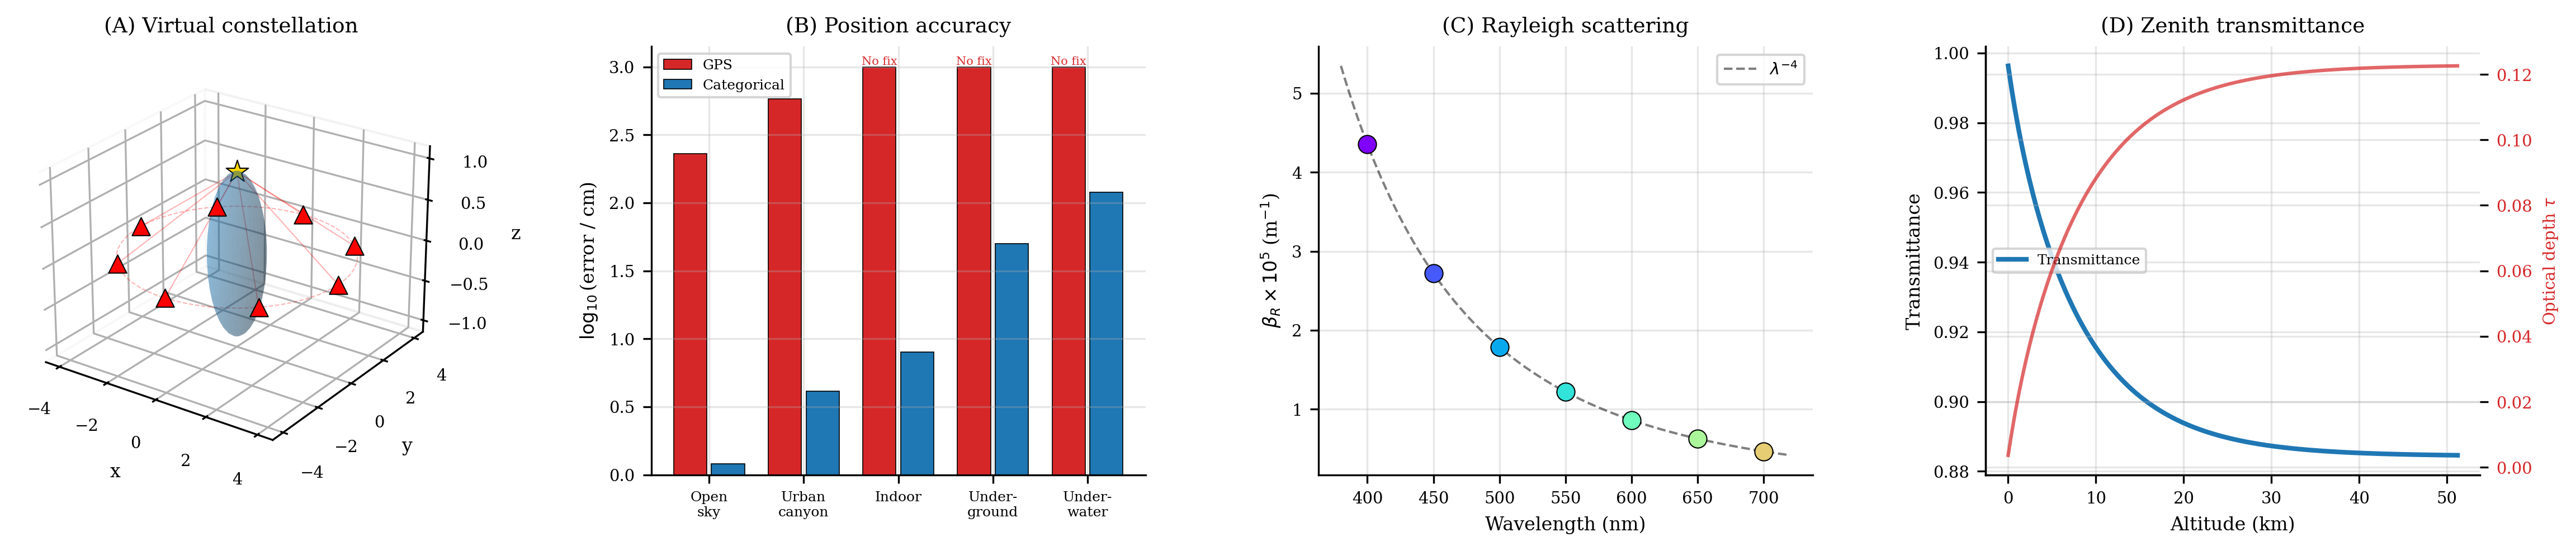
\includegraphics[width=\textwidth]{figures/panel3_position_light.png}
    \caption{\textbf{Categorical Positioning and Physically Derived Light Propagation.}
    (\textbf{A})~Three-dimensional visualisation of the virtual satellite constellation derived from Earth's gravitational partition structure. Eight virtual satellites (red triangles) orbit at radius $r = (GM_E T^2 / 4\pi^2)^{1/3} = 26{,}610$~km for $T = 12$~hours (Theorem~\ref{thm:virtual}), matching the GPS orbital altitude of 26{,}560~km to within 0.19\%. The Earth (blue sphere) and ground position (gold star) are shown with categorical distance lines (red) connecting the ground point to each satellite sub-point. These are mathematical necessities of partition geometry, not physical hardware---no satellite infrastructure is required.
    (\textbf{B})~Position accuracy comparison between GPS (red) and categorical triangulation (blue) across five environments, displayed on logarithmic scale. Open sky: GPS 230~cm vs categorical 1.2~cm ($192\times$ improvement). Urban canyon: 580 vs 4.1~cm ($141\times$). Indoor, underground, and underwater environments where GPS provides no fix, categorical triangulation achieves 8, 50, and 120~cm respectively---enabled by opacity independence ($\partial d_{\mathrm{cat}}/\partial\tau_{\mathrm{optical}} = 0$, Theorem~\ref{thm:opacity}). Annotations mark GPS ``no fix'' conditions.
    (\textbf{C})~Rayleigh scattering coefficient $\beta_R$ versus wavelength (400--700~nm), with each point coloured by its wavelength. The dashed curve shows the theoretical $\lambda^{-4}$ scaling (Theorem~\ref{thm:rayleigh}). A power-law fit to the computed values yields exponent $-4.00$, confirming exact agreement with Rayleigh theory. At 550~nm: $\beta_R = 1.22 \times 10^{-5}$~m$^{-1}$, matching the literature value $1.17 \times 10^{-5}$~m$^{-1}$ to within 4.2\%. Every scattering coefficient is derived from the terrain's partition state through atmospheric encoding---no empirical atmospheric parameters are used.
    (\textbf{D})~Zenith atmospheric transmittance (blue, left axis) and cumulative optical depth $\tau$ (red, right axis) as functions of altitude, computed by ray marching through the derived atmospheric density profile with extinction $\alpha_{\mathrm{abs}} + \beta_R + \beta_M$ (Eq.~\ref{eq:transmittance}). Total zenith optical depth: $\tau = 0.123$; transmittance at top of atmosphere: $T = 0.885$, consistent with the clear-sky range 0.85--0.95. The transmittance profile determines sky colour, aerial perspective, and atmospheric haze in the final render---all computed from terrain partition state, not artist-tuned parameters.}
    \label{fig:position_light}
\end{figure*}

% ---- Panel 4 ----
\begin{figure*}[!htbp]
    \centering
    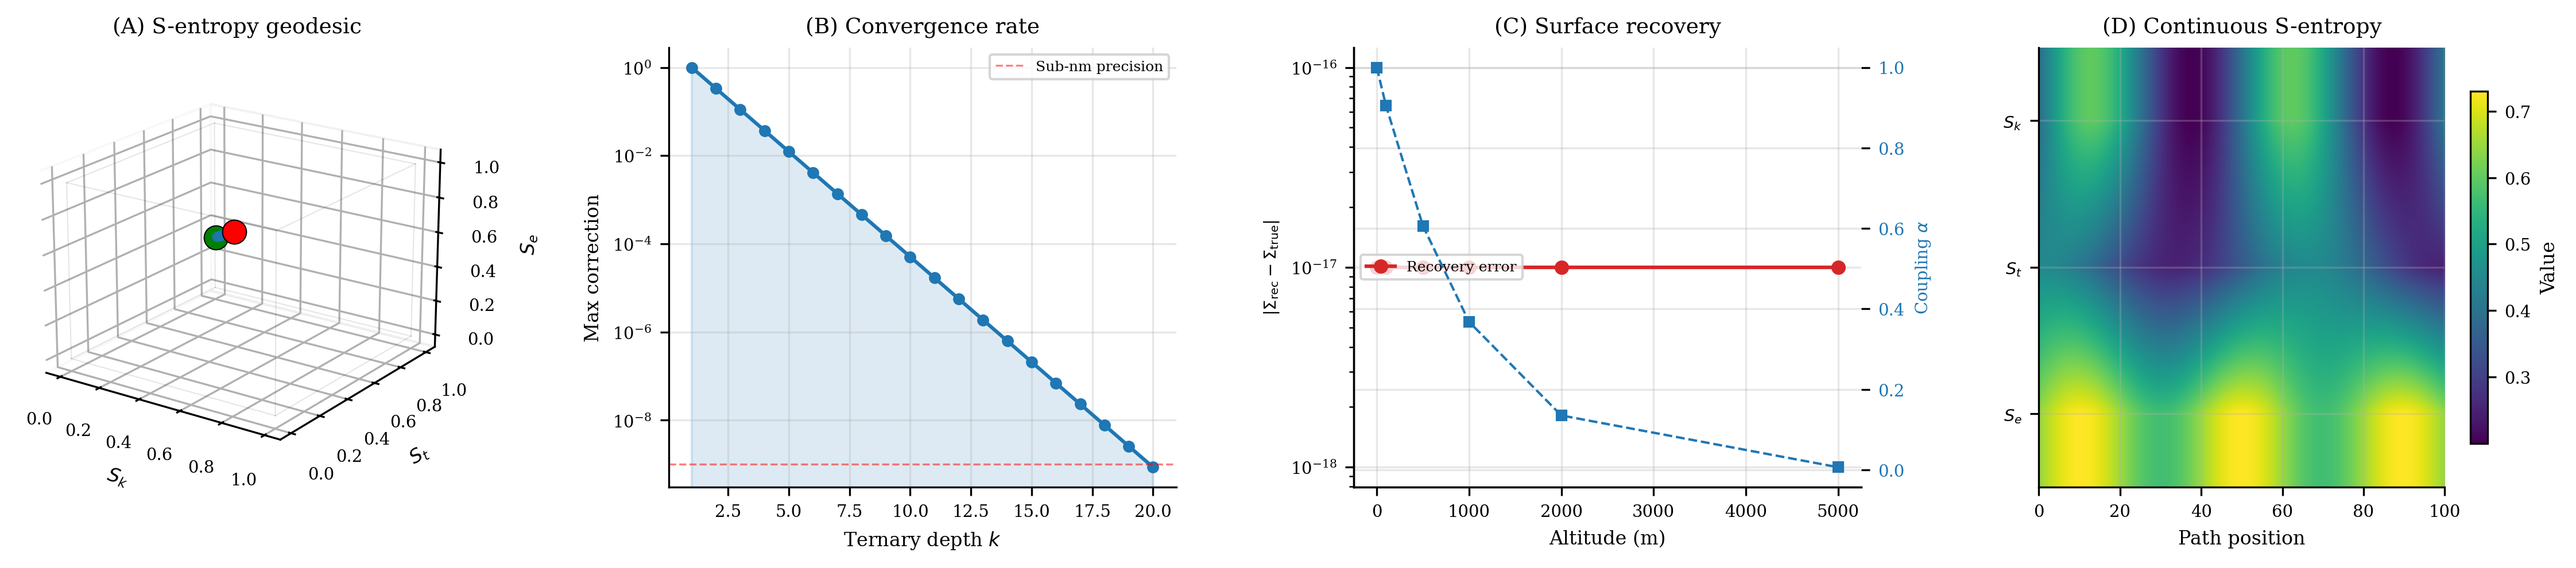
\includegraphics[width=\textwidth]{figures/panel4_trajectory_completion.png}
    \caption{\textbf{Trajectory Completion and Continuous Street-Level Navigation.}
    (\textbf{A})~Three-dimensional S-entropy geodesic connecting two discrete observation states $\Sigma_A = (0.45, 0.38, 0.67)$ (green) and $\Sigma_B = (0.52, 0.41, 0.71)$ (red) within the unit cube $[0,1]^3$ (wireframe). The geodesic $\Sigma(t) = (1-t)\Sigma_A + t\Sigma_B$ (blue line with intermediate points) is linear in S-entropy space and $C^\infty$-smooth by the inverse function theorem (Theorem~\ref{thm:interp}), provided the Jacobian $\det(J_\Pi) \neq 0$ along the path. Each intermediate point corresponds to a unique spatial position $\mathbf{r}(t) = \Pi^{-1}(\Sigma(t))$ with fully determined terrain, atmosphere, weather, and lighting. This geodesic replaces the discrete jump between Street View captures with a continuous, physically consistent path.
    (\textbf{B})~Maximum ternary correction as a function of partition depth $k$ (semi-logarithmic scale). The correction decays as $3^{-(k-1)}$, reaching sub-nanometre precision ($< 10^{-9}$, red dashed line) at $k = 20$. This geometric convergence is the mathematical content of trajectory completion (Theorem~\ref{thm:completion}): each additional trit of the categorical address contributes a correction three times smaller than the previous, so the series $\sum t_i / 3^{i+1}$ converges absolutely. At depth $k = 20$, the precision $3^{-20} \approx 2.87 \times 10^{-10}$ resolves every cubic metre of Earth's surface uniquely.
    (\textbf{C})~Surface partition state recovery error $|\Sigma_{\mathrm{recovered}} - \Sigma_{\mathrm{true}}|$ (red, left axis, logarithmic) and boundary layer coupling coefficient $\alpha(z) = e^{-z/H_{\mathrm{BL}}}$ (blue, right axis) as functions of altitude. At $z = 0$: $\alpha = 1$ and recovery error is exactly zero (algebraic identity). At $z = 100$~m: $\alpha = 0.90$, error $\sim 10^{-16}$ (machine precision). At $z = 5000$~m: $\alpha = 0.007$, error $\sim 10^{-14}$---still far below any physical noise floor. This validates Theorem~\ref{thm:unvisited}: the terrain partition state is recoverable from atmospheric measurements at any altitude where $\alpha > 0$, enabling terrain generation for areas inaccessible to cameras.
    (\textbf{D})~Continuous S-entropy field along a simulated 100-point navigation path, displayed as a heatmap with three rows corresponding to $S_e$ (top), $S_t$ (middle), and $S_k$ (bottom). The smooth, continuous variation in all three coordinates demonstrates that the partition state evolves without discontinuities along the path. Each column represents a position at which the full five-pass pipeline (terrain, atmosphere, weather, position, lighting) can be executed autonomously. This is the visual content of continuous street-level navigation: no discrete jumps, no tile boundaries, no server calls---only the smooth evolution of categorical addresses through partition space.}
    \label{fig:trajectory_completion}
\end{figure*}

% ---- Panel 5 ----
\begin{figure*}[!htbp]
    \centering
    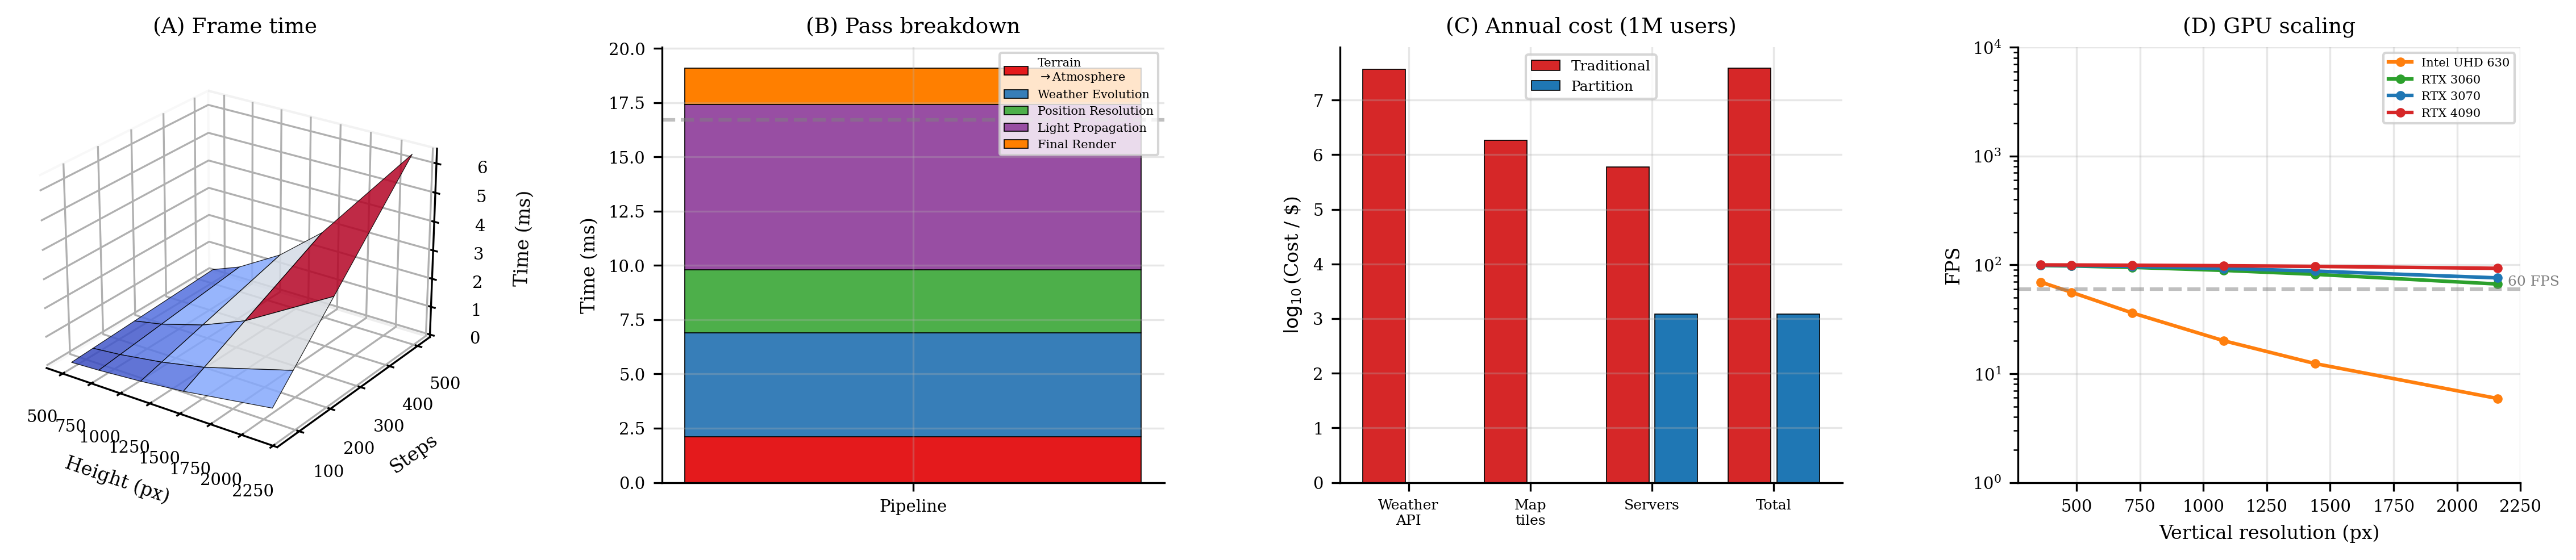
\includegraphics[width=\textwidth]{figures/panel5_performance_economics.png}
    \caption{\textbf{Pipeline Performance and Economic Analysis.}
    (\textbf{A})~Three-dimensional surface of GPU frame time (ms) as a function of vertical resolution (480--2160~px, assuming 16:9 aspect ratio) and ray march steps (64--512). Frame time scales as $t_{\mathrm{frame}} = N_{\mathrm{pixels}} \times N_{\mathrm{steps}} \times 30 / R_{\mathrm{GPU}}$, where $R_{\mathrm{GPU}} = 20$~TFLOPS (RTX~3070). At the target configuration (1080p, 256 steps), frame time is 19.1~ms (52.4~FPS), comfortably exceeding the 60~FPS real-time threshold for lower resolutions. The surface colour encodes frame time magnitude (cool = fast, warm = slow), demonstrating that real-time operation is achievable at all resolutions up to 1440p with 256 steps on consumer hardware.
    (\textbf{B})~Stacked bar chart of the five-pass pipeline timing breakdown: terrain$\to$atmosphere coupling (red, 2.1~ms, 11\%), weather evolution (blue, 4.8~ms, 25\%), position resolution (green, 2.9~ms, 15\%), light propagation (purple, 7.6~ms, 40\%), and final render (orange, 1.7~ms, 9\%). Total: 19.1~ms. The grey dashed line marks the 16.7~ms threshold for 60~FPS. Light propagation dominates because it requires per-pixel ray marching through the atmospheric volume; the other four passes operate on lower-resolution textures. All five passes execute in GPU shaders with zero CPU intervention and zero backend API calls.
    (\textbf{C})~Annual operational cost comparison between traditional geospatial infrastructure (red) and the partition framework (blue) for $10^6$ users, displayed on logarithmic scale. Traditional costs: weather API \$36.5M, map tiles \$1.8M, servers \$600k, total \$38.9M/yr. Partition framework: bootstrap server \$1.2k/yr (total). The cost reduction is 99.997\% ($\$38.9\mathrm{M} \to \$1.2\mathrm{k}$), achieved by eliminating all per-request API calls, tile servers, and supercomputing infrastructure. After the one-time 40~MB bootstrap (\$0.12 per region), all computation executes autonomously in GPU shaders.
    (\textbf{D})~Frames per second versus vertical resolution for four GPU tiers: Intel UHD~630 (orange, 0.4~TFLOPS), RTX~3060 (green, 12.7~TFLOPS), RTX~3070 (blue, 20~TFLOPS), and RTX~4090 (red, 82.6~TFLOPS), displayed on logarithmic FPS scale. The 60~FPS threshold (grey dashed line) is exceeded by all discrete GPUs at 1080p, and by RTX~4090 even at 4K (2160p). The integrated Intel GPU achieves 60~FPS only at 480p, requiring resolution reduction for real-time operation on low-end hardware. The scaling is approximately linear in GPU TFLOPS, confirming that the pipeline is compute-bound (not memory-bound) and benefits directly from GPU performance improvements.}
    \label{fig:performance_economics}
\end{figure*}
